\documentclass[aspectratio=169,11pt]{beamer}

\usetheme{Madrid}
\usecolortheme{default}
\usefonttheme{professionalfonts}
\setbeamertemplate{navigation symbols}{}
\setbeamertemplate{footline}[frame number]

\usepackage{amsmath, amssymb, booktabs, graphicx}
\graphicspath{{../../assets/figures/}{assets/figures/}}

\title{Aggregate Fluctuations and Labor Market Adjustment}
\subtitle{Labor II --- Week 10}
\author{Teaching deck draft}
\date{}

\begin{document}

\begin{frame}
  \titlepage
\end{frame}

\begin{frame}{Central question and week repositioning}
\begin{itemize}
    \item When aggregate conditions weaken or strengthen, which labor-market margins do the adjusting?
    \item Week 10 scales Week 4 search objects and Week 9 institutional margins up to economy-wide shocks.
    \item The lecture stays labor-focused: unemployment, vacancies, separations, job-to-job mobility, wages, and match quality.
\end{itemize}
\end{frame}

\begin{frame}{Week 9 to Week 10 bridge}
\begin{itemize}
    \item Week 9: regulation, enforcement, and insurance shape layoffs, recalls, search, and vacancy posting.
    \item Week 10: the same margins move when shocks are aggregate rather than policy-specific.
    \item Week 11 will keep these margins in view but switch from cyclical adjustment to structural technology shocks.
\end{itemize}
\end{frame}

\begin{frame}{Stocks, flows, and hidden margins}
\begin{center}
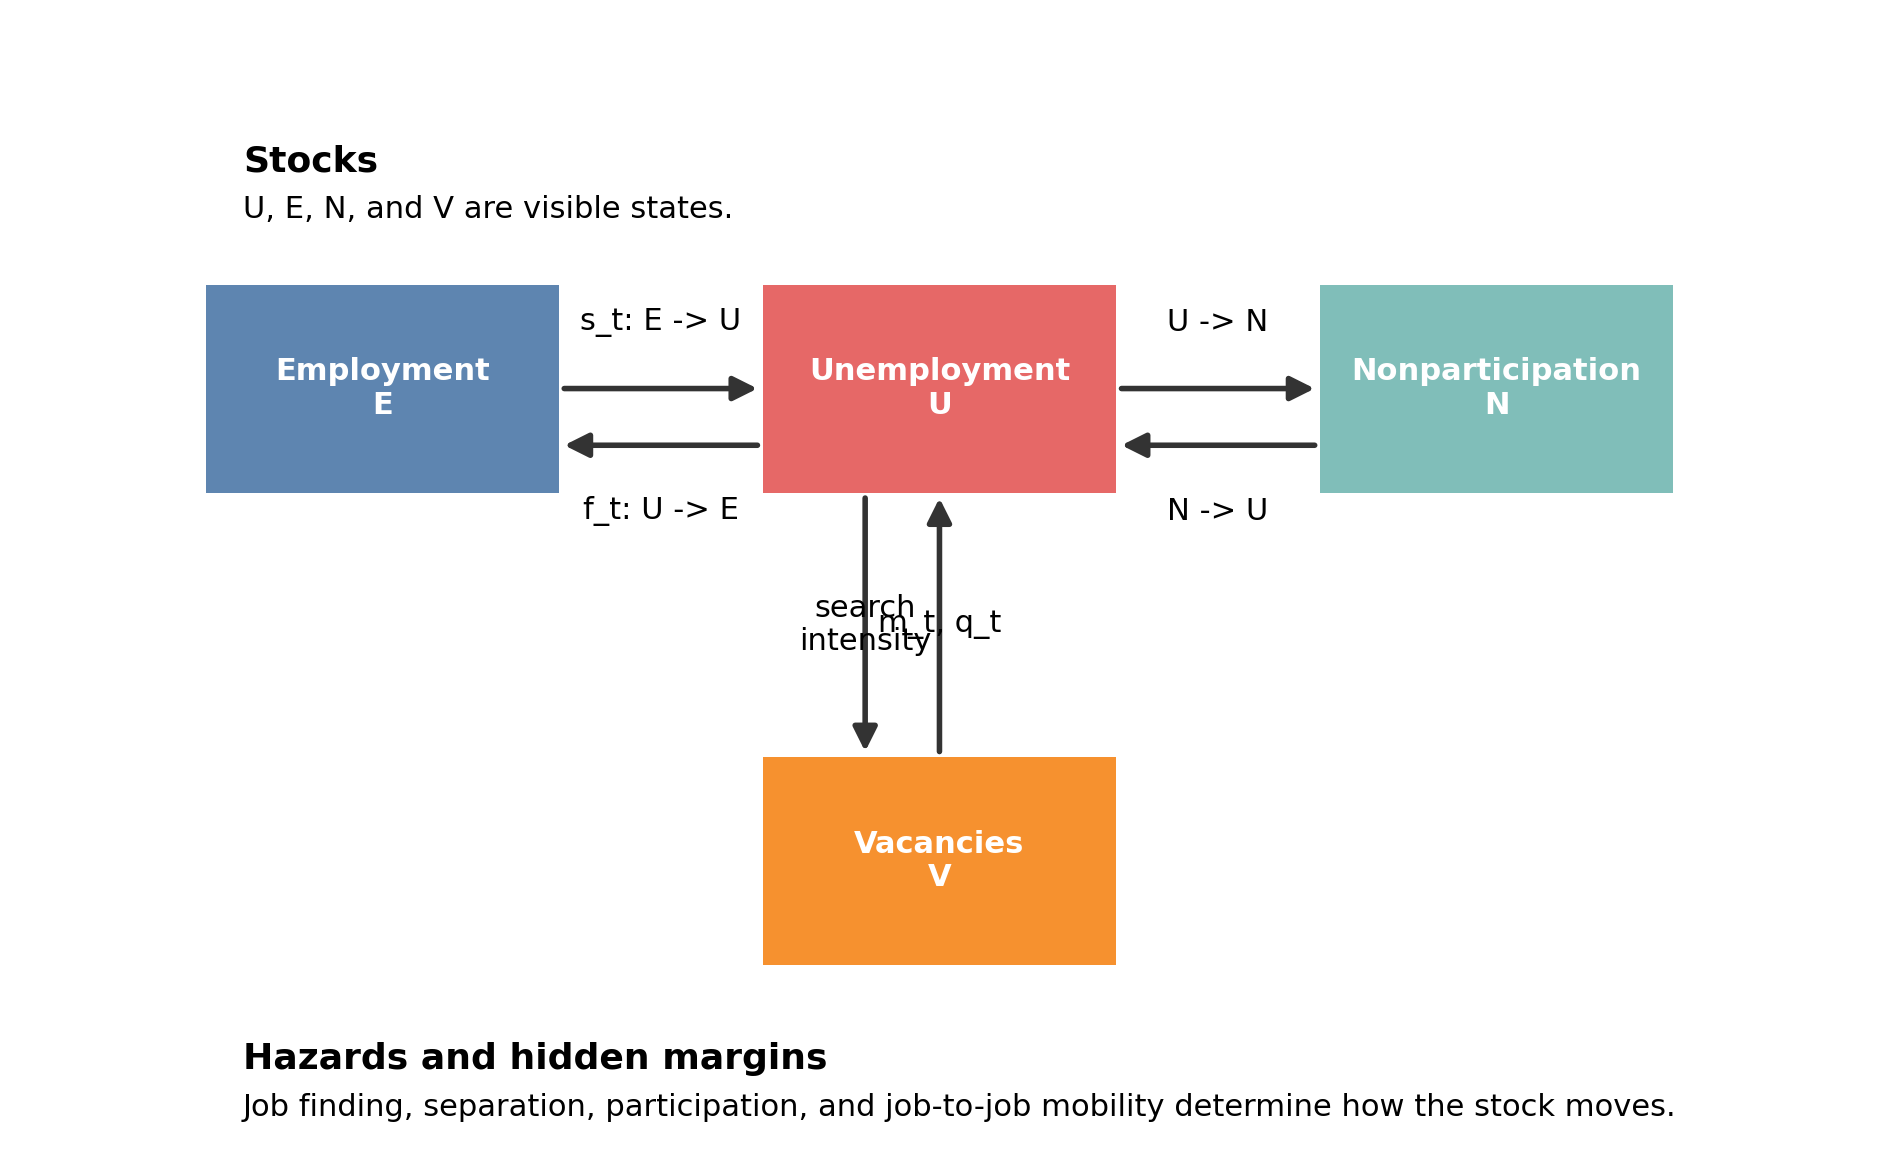
\includegraphics[height=0.73\textheight]{10-aggregate-flows-and-margins.png}
\end{center}
\end{frame}

\begin{frame}{Labor-market stocks and the law of motion for unemployment}
\[
\dot u_t = s_t(1-u_t) - f_t u_t,
\qquad
u_t^{\ast} = \frac{s_t}{s_t + f_t}
\]

\begin{itemize}
    \item Unemployment is a stock.
    \item Job finding $f_t$ and separation $s_t$ are hazards.
    \item A high unemployment rate can come from high inflows, low outflows, or both.
\end{itemize}
\end{frame}

\begin{frame}{Three-state extension and hidden slack}
\[
\begin{pmatrix}
E_{t+1}\\
U_{t+1}\\
N_{t+1}
\end{pmatrix}
=
P_t
\begin{pmatrix}
E_t\\
U_t\\
N_t
\end{pmatrix}
\]

\begin{itemize}
    \item The $E/U/N$ system keeps participation margins visible.
    \item A pure two-state unemployment narrative can miss hidden slack and attachment dynamics.
    \item Gross worker flows matter for aggregate labor adjustment, not only the unemployment rate.
\end{itemize}
\end{frame}

\begin{frame}{Matching, tightness, and the Beveridge curve}
\[
m_t = \mu_t u_t^{\alpha} v_t^{1-\alpha},
\qquad
f_t = \frac{m_t}{u_t} = \mu_t \theta_t^{1-\alpha},
\qquad
q_t = \frac{m_t}{v_t} = \mu_t \theta_t^{-\alpha}
\]

\begin{itemize}
    \item Tightness $\theta_t = v_t/u_t$ links worker-side and vacancy-side hazards.
    \item Workers care about $f_t$; firms care about $q_t$.
    \item Beveridge-curve shifts need not identify one primitive.
\end{itemize}
\end{frame}

\begin{frame}{Matching residuals and Beveridge-curve interpretation}
\[
\mu_t = \frac{m_t}{u_t^{\alpha} v_t^{1-\alpha}},
\qquad
u_t^{\ast} = \frac{s_t}{s_t + \mu_t \theta_t^{1-\alpha}}
\]

\begin{center}
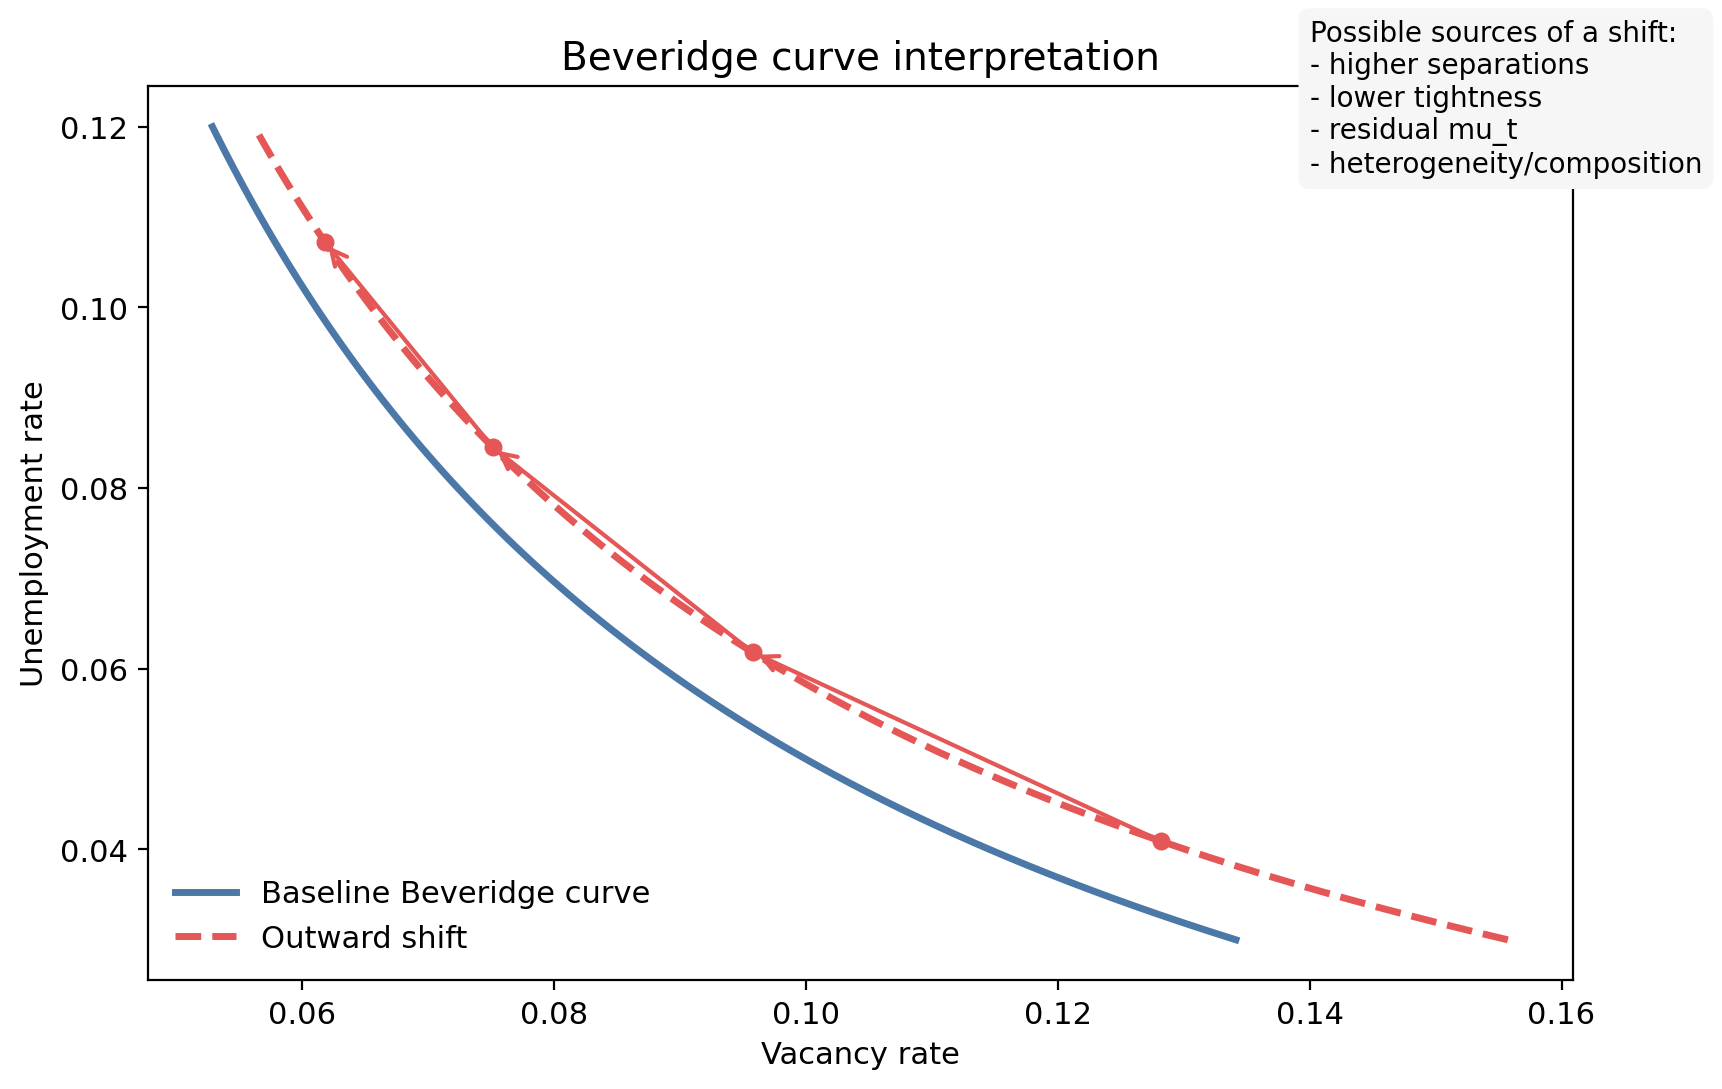
\includegraphics[height=0.53\textheight]{10-beveridge-curve-and-matching-efficiency.png}
\end{center}
\end{frame}

\begin{frame}{Free entry, surplus, and the Shimer-Hall logic}
\[
\kappa = q_t \, \mathbb{E}_t[J_{t+1}],
\qquad
S_t = J_t + W_t - U_t
\]

\begin{itemize}
    \item Vacancy creation depends on expected surplus.
    \item Shimer: benchmark shocks do not move surplus enough to match vacancy and unemployment volatility.
    \item Hall: wage stickiness keeps wages from absorbing the whole shock and amplifies vacancy posting.
\end{itemize}
\end{frame}

\begin{frame}{Unemployment stocks versus flows}
\[
\Delta u_t \approx (1-u_t)\Delta s_t - u_t \Delta f_t
\]

\begin{itemize}
    \item Elsby-Michaels-Solon: cyclical unemployment is an inflow-outflow object.
    \item Severe recessions often involve both weaker job finding and higher separations.
    \item CPS-style decompositions observe transition hazards, then infer contributions to the stock.
\end{itemize}
\end{frame}

\begin{frame}{Separations, endogenous destruction, and churning}
\[
s_t = \Pr\!\left(S_t(z) < 0\right),
\qquad
\text{Churning}_t = \text{Worker Reallocation}_t - \text{Job Reallocation}_t
\]

\begin{center}
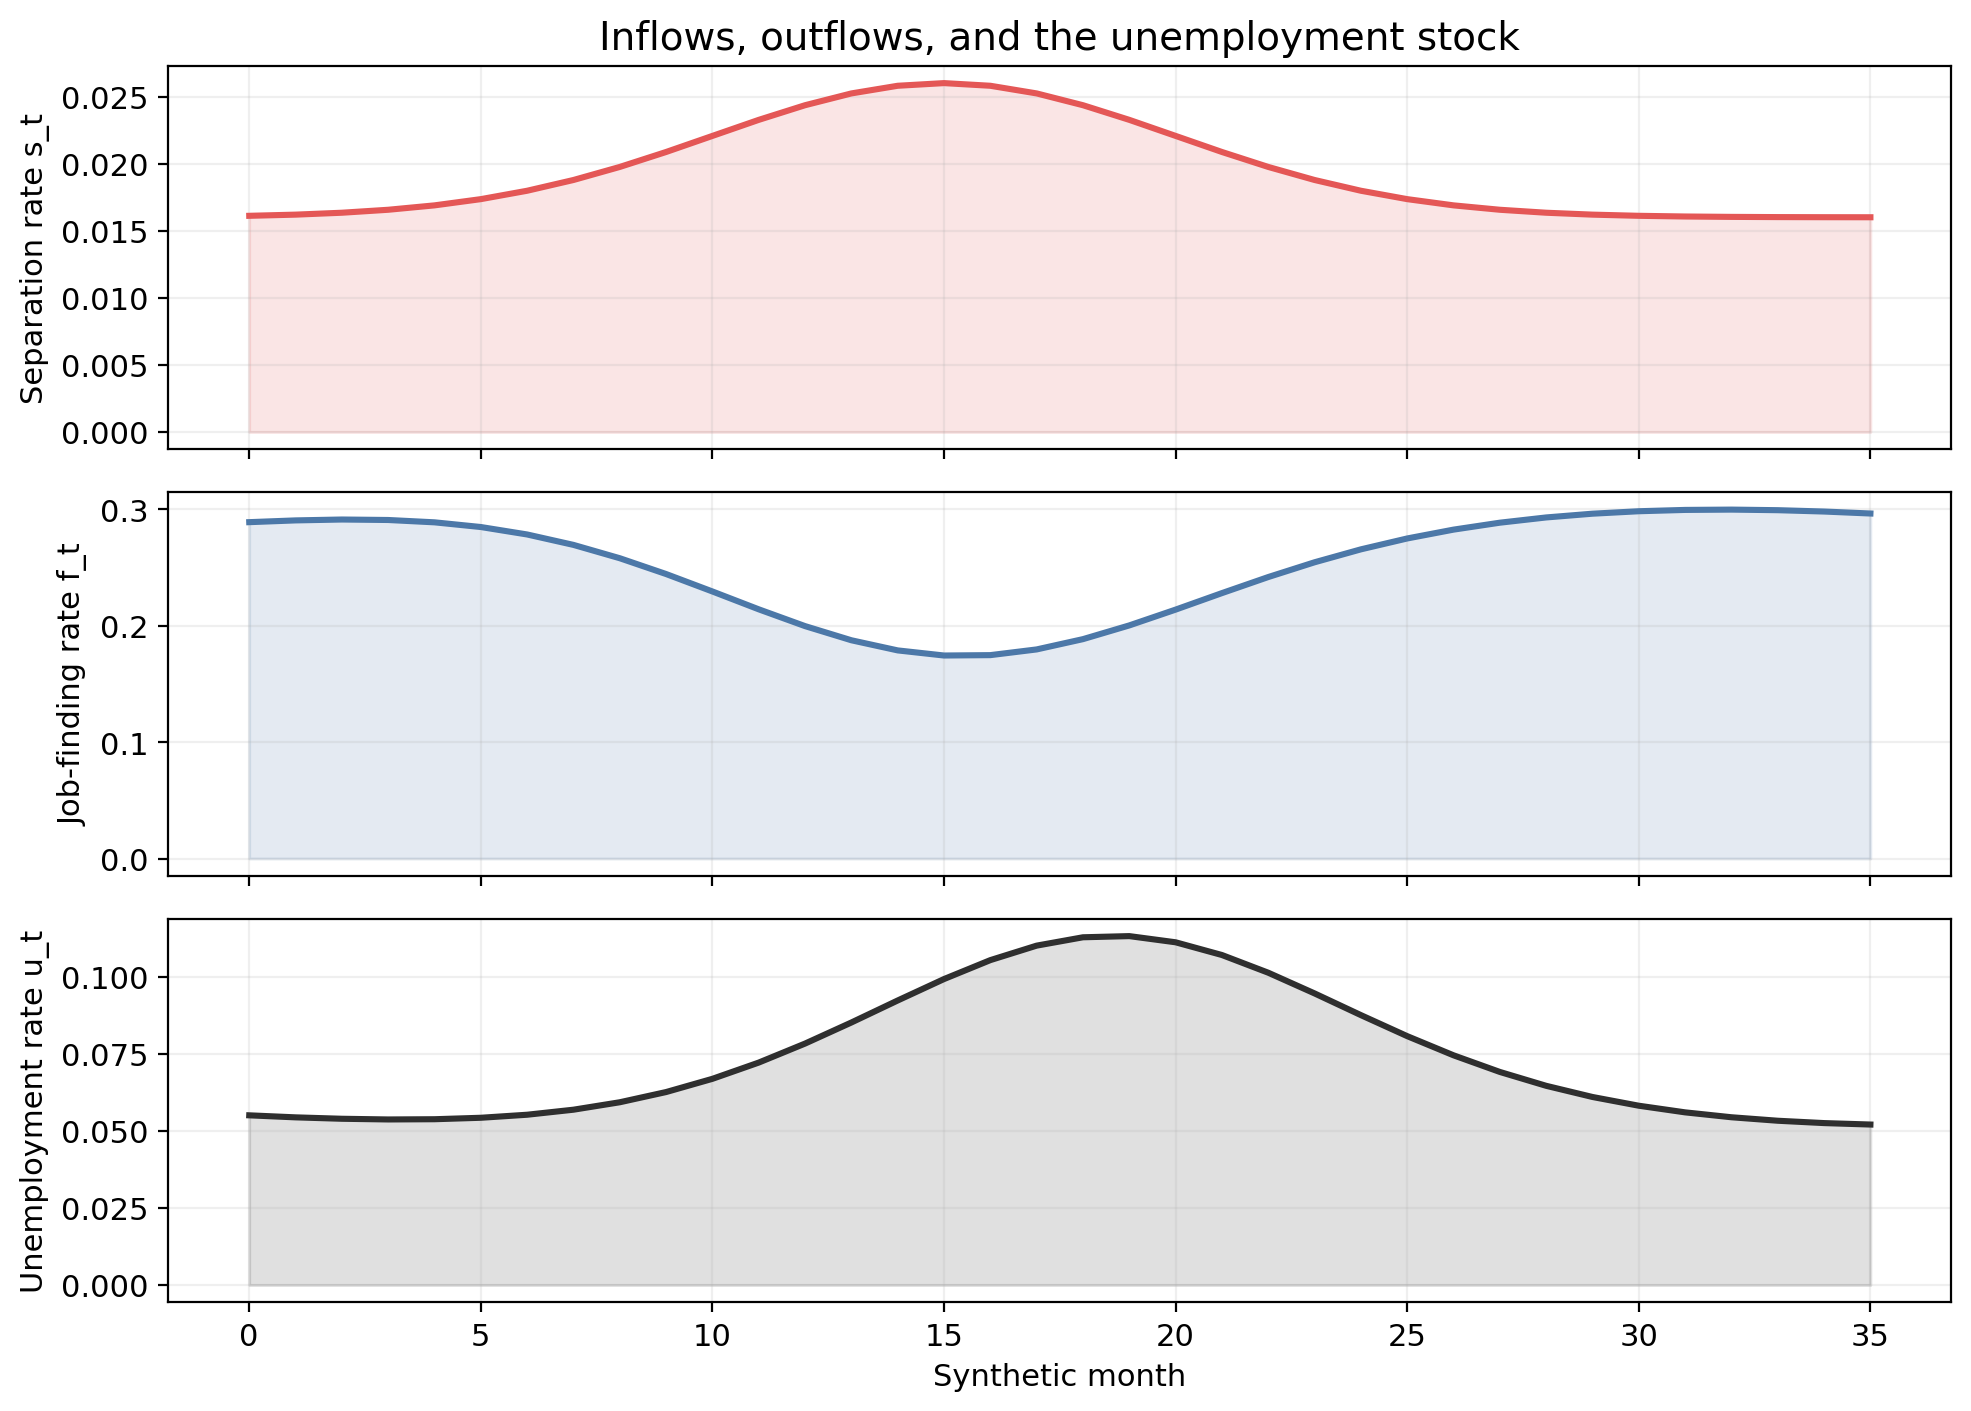
\includegraphics[height=0.50\textheight]{10-separations-jobfinding-unemployment.png}
\end{center}
\end{frame}

\begin{frame}{On-the-job search, job-to-job transitions, and churning}
\[
EE_t = \lambda_t^{e}\Pr\!\left(w' > w\right)
\]

\begin{itemize}
    \item Aggregate labor adjustment is not only unemployment.
    \item Job ladders flatten in weak markets when outside offers collapse.
    \item Reallocation among employed workers is a wage and match-quality margin.
\end{itemize}

\begin{center}
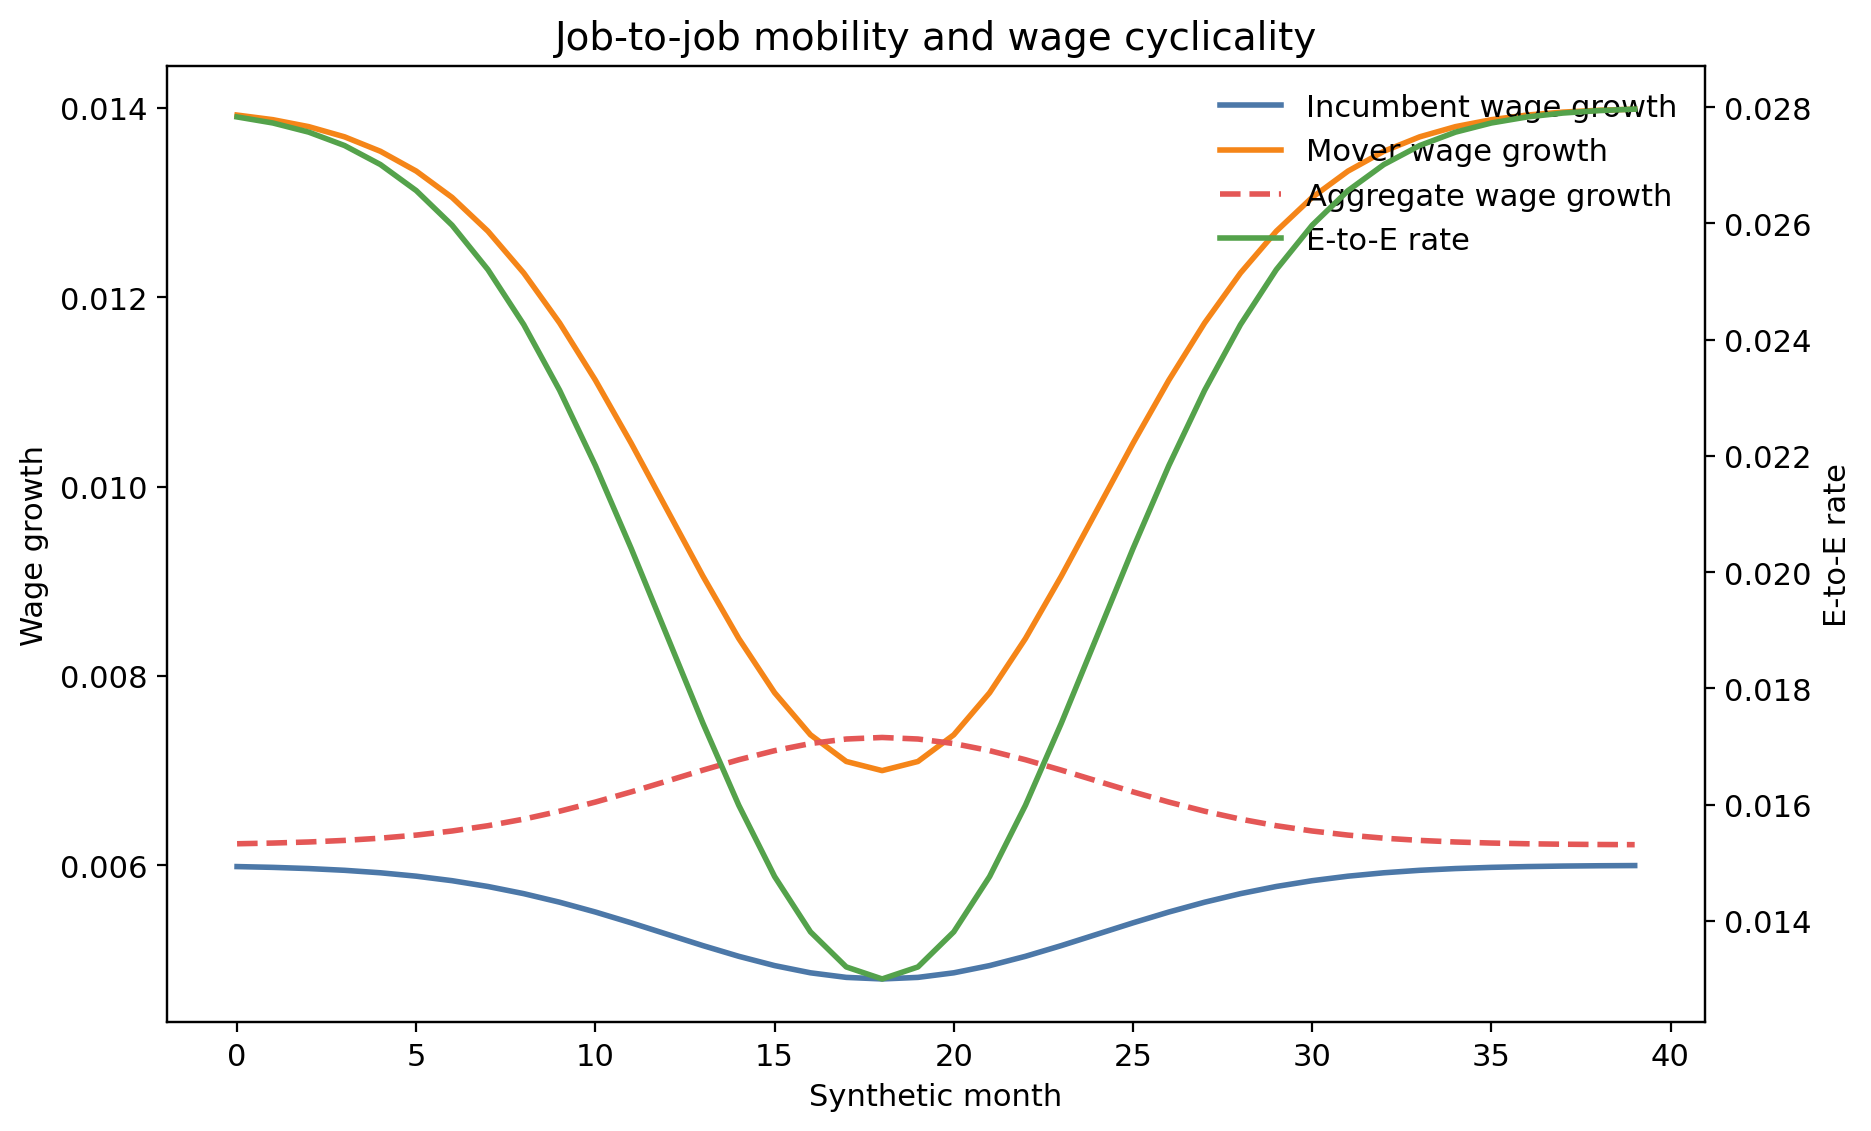
\includegraphics[height=0.34\textheight]{10-job-to-job-wage-cyclicality.png}
\end{center}
\end{frame}

\begin{frame}{Wage cyclicality, sorting, and match quality}
\[
\Delta \log \bar w_t =
\beta^{I} \, cyc_t
+ \omega_t^{EE}\beta^{EE} \, cyc_t
+ comp_t + sort_t
\]

\begin{itemize}
    \item Incumbent wage cyclicality is not the same object as mover wage cyclicality.
    \item Average wage growth is contaminated by selection and sorting.
    \item Weak measured wage cyclicality may hide strong movements in outside offers and match quality.
\end{itemize}
\end{frame}

\begin{frame}{Match quality and cyclical reallocation}
\begin{center}
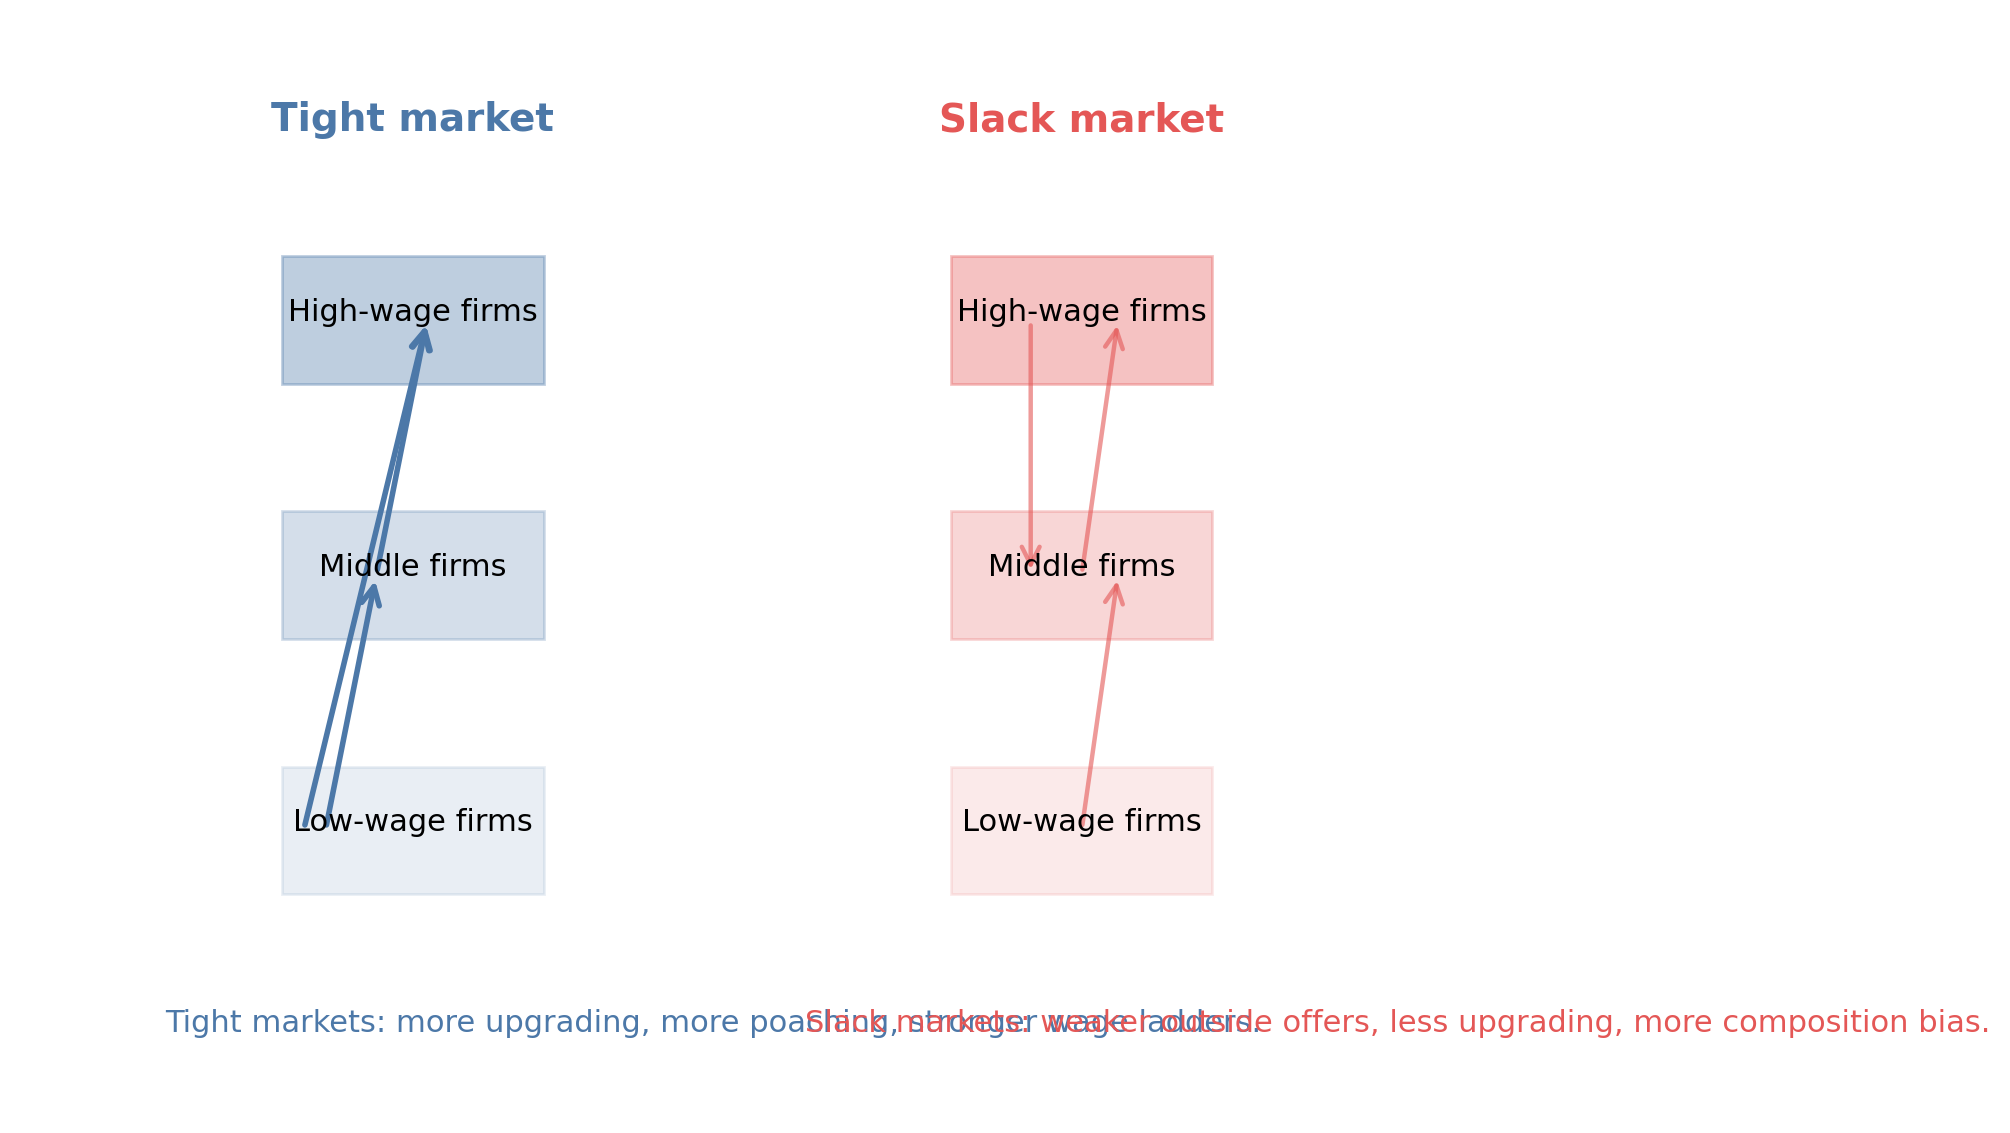
\includegraphics[height=0.72\textheight]{10-match-quality-and-reallocation.png}
\end{center}
\end{frame}

\begin{frame}{Empirical designs and what they identify}
\small
\begin{tabular}{p{0.20\linewidth} p{0.18\linewidth} p{0.23\linewidth} p{0.26\linewidth}}
\toprule
Design & Unit & Observed margin & Main hidden margin \\
\midrule
National time series & market-time cell & $U$, $V$, hires, flows & composition and segmentation \\
Stock-flow decomposition & worker-state transitions & $U{\to}E$, $E{\to}U$, $U$ stock & recall, misclassification, job quality \\
State/local cyclicality & area-time cell & unemployment, wages, vacancies & aggregate equilibrium mechanism \\
Matched employer-employee data & worker-firm spell & $E{\to}E$, separations, wage ladder & full opportunity set and GE response \\
\bottomrule
\end{tabular}
\end{frame}

\begin{frame}{Recent Beveridge-curve-shift evidence and open questions}
\begin{itemize}
    \item A matching residual is not enough: heterogeneity, search intensity, and vacancy composition all matter.
    \item Why do Beveridge-curve shifts differ across eras?
    \item How much cyclical adjustment runs through recalls, temporary layoffs, and participation margins?
    \item How much measured wage rigidity is really sorting or match-quality change?
\end{itemize}
\end{frame}

\begin{frame}{Bridge to Week 11 technology and adjustment}
\begin{itemize}
    \item Week 10: cyclical shocks move hazards, vacancies, mobility, and wages over the business cycle.
    \item Week 11: technology, automation, and AI move many of the same labor-market objects through more persistent restructuring.
    \item The labor-market margins stay the same even when the shock changes.
\end{itemize}
\end{frame}

\begin{frame}{Takeaways}
\begin{itemize}
    \item Unemployment is a stock governed by multiple hazards.
    \item Matching, separation, and job-to-job mobility are distinct cyclical margins.
    \item Beveridge-curve shifts and wage cyclicality are hard to interpret without composition and sorting.
    \item Aggregate labor adjustment is a map of labor-market objects, not a single macro fact.
\end{itemize}
\end{frame}

\appendix

\begin{frame}{Appendix: Week 10 lab bridge}
\begin{itemize}
    \item Reproduce: a Barnichon-Figura-style aggregate matching exercise.
    \item Diagnose: an Elsby-Michaels-Solon-style unemployment stock-flow decomposition.
    \item Transfer: a small job-to-job and wage-cyclicality exercise.
    \item Keep the object explicit: stock, hazard, efficiency residual, or job ladder.
\end{itemize}
\end{frame}

\end{document}
